%!TEX root = ../proceedings.tex
% \subsection{Feedback}
\textit{Ratings cause anxiety, whereas feedback can satisfy the same administrative needs without causing workers undue stress.}

At organization E, we learned that workers interpreted negative feedback very personally,
making it difficult for them to internalize that feedback constructively and act on the suggestions customers made.
Multiple issues may have been at play here;
cultural differences might explain a mismatch in how feedback is offered and how it is received,
but so too would the power imbalance between undocumented domestic workers and their customers.

organization E didn't seem to investigate the cause of this effect,
but their solution circumvented this problem entirely.
Rather than giving workers unfiltered, raw feedback as it streamed in,
organization E intercepted reviews from customers and distilled them into constructive, actionable feedback.
Both praise and criticism would sometimes be read aloud to the entire group,
with identifying information removed.

\begin{figure}[t]
\centering
  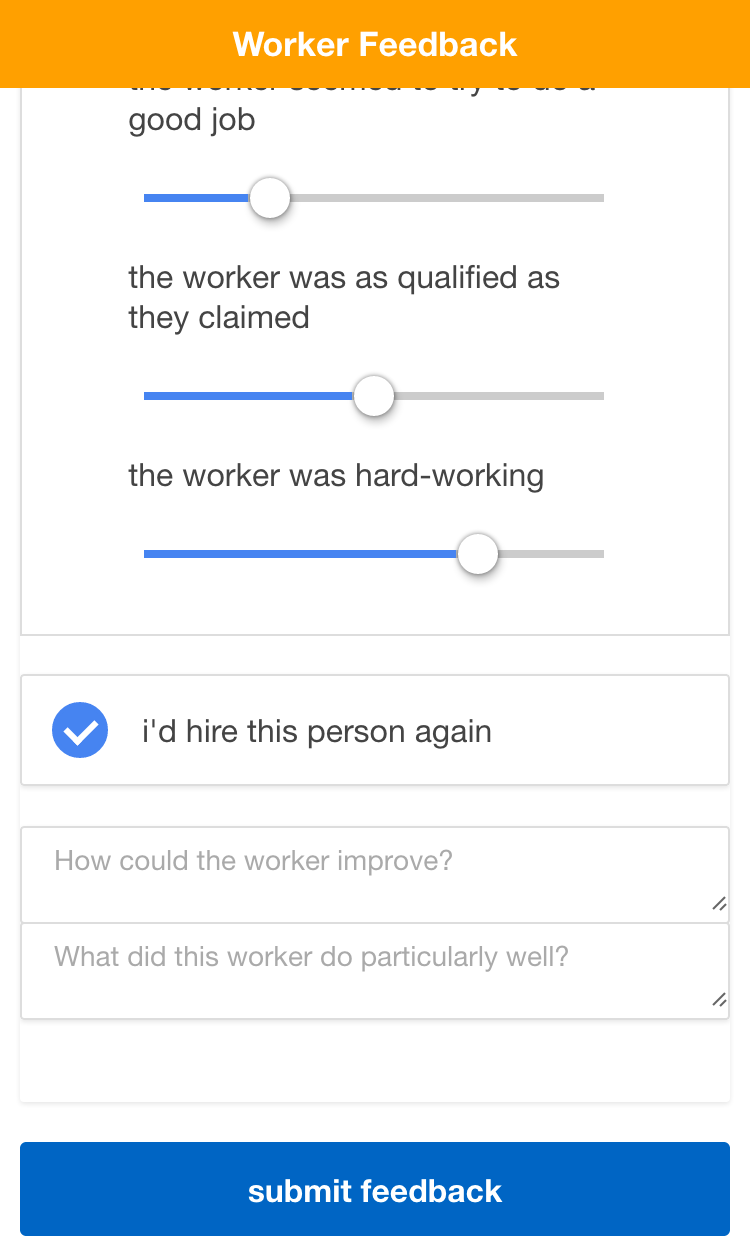
\includegraphics[width=1\columnwidth]{figures/feedback}
    \caption{Given quantitative prompts and qualitative follow-up questions,
  research suggests that users are more likely to write more,
  which can better-inform.}~\label{fig:workerFeedback}
\end{figure}

The purpose of reading positive feedback publicly was to reaffirm the group's sense of worth in a shared sense of success;
the purpose of reading the negative feedback, meanwhile, was to prompt workers to reflect on what went ``wrong'', and how to avoid such an outcome in the future.
A shared sense of failure also seemed to affect workers in these cases;
whether this is an outcome of public readings of reviews, or more complex relationships between workers and organization E, is unclear.

Speaking with Uber and Lyft drivers, we found an alternative approach to providing workers with feedback;
drivers are made aware of an aggregated rating
--- generally a moving average of the previous \textit{n} ratings ---
but they are not exposed to qualitative feedback in any form, even when customers provide it.

A driver's current aggregated rating, it turns out, is extremely important:
a driver's rating determines the worker's eligibility to do work, and falling below various thresholds carries various consequences. Reports suggesting that these thresholds are finely tuned as well as closely guarded secrets make these markets particularly emotionally taxing for workers \cite{leakedUber}.

When we spoke to drivers, they relayed stories of apparent obligations to take expensive remedial courses if their overall rating dropped below a certain threshold,
and widely held fears of suspension and deactivation for falling below an unknown level weigh heavily on workers' minds.
Frustration directed at drunk, clumsy, or naive passengers accidentally or deliberately giving drivers a rating of 4 (out of 5) stars further exacerbates stress.

Markets which aim to empower ``gig workers'' should use quantitative rating systems sparingly,
or to prompt more detailed qualitative feedback, as we illustrate in Figure
\ref{fig:workerFeedback}.
Quantitative ratings in the form of Likert scales followed by qualitative prompts for feedback seem to precipitate more detailed feedback
\cite{numericCritique}.

% While quantitative metrics
% --- like approval rates and moving average ratings ---
% make large-scale evaluation seemingly manageable and generalizable,
% the professional stress these
Quantitative metrics --- especially those that are opaquely evaluated --- do not benefit workers, nor does it seem they even inform appropriate customer behavior \cite{ebayRatings}.
Meanwhile, constructive feedback suggesting improvements may provide workers with the necessary information to improve as professionals without causing undue stress over issues such as worker eligibility..